\chapter{系统总体设计}
\section{目标分析}
本小节主要分析了Rails消息总线项目的具体需求。本项目由三个子项目构成,Rails消息总线子项目用于提供从Rails服务器到浏览器的基础服务技术;Auto-Reload技术主要用于开发模式时自动检测源代码更改事件并通知浏览器进行刷新动作;而Backend Instrumentation技术则是通过在后台采集性能数据,并将其反馈到前端的技术。

\subsection{Rails消息总线需求分析}
Rails消息总线提供了一套机制,使得服务器能够实时地推送任意数据到浏览器客户端。本文从两个层面上实现了Rails消息总线技术,这两个层面抽象程度、易用性以及灵活性各不相同,适应于不同的应用场景。针对这两个层面,Rails消息总线技术提供了两套接口(模式)。 这两套接口中,抽象程度较低、更为灵活的是Raw Streaming Mode,使用这套接口,服务器可以发送任意格式的数据,HTTP报文的报头和内容完全由服务器定制而不受Rails框架限制。另一套接口是SSE Mode,该套接口抽象程度较高,使用更为简单。SSE Mode即Server Sent Events技术的Rails实现版本,Rails消息总线技术实现了较为完整的SSE技术规范,对于规范中大部分内容(特别是开发环境中最常使用的特性)都予以了支持。

对于Raw Streaming模式,Rails消息总线技术允许程序获取服务器和浏览器连接的原始套接字对象。并且允许开发者直接向该套接字读写数据,并且写入的数据将被即刻传输至浏览器,从而实现了实时数据推送。为了使得服务器能够推送数据,首先需要浏览器主动连接到Rails服务器上以获取数据。该过程需要通过浏览器向Rails服务器发送一个传统的HTTP连接请求来完成,因此在服务器端,开发者必须首先定义一个入口Controller和相应的action。当入口Controller和action定义好,并且在Rails项目的route.rb文件中注册完成之后,浏览器可以通过地址“http://server\_addr/controller/action”连接上Rails服务器。此时由于该路径已在route.rb中注册成功,Rails会将该请求路由到相应的Controller及其action上的代码处。此时,Rails开发者可以通过在相应的action中获取response对象,通过向数据流response.stream写入数据,可以实现超浏览器发送实时数据。代码\ref{raw-streaming-demo}展示了如何使用该接口:

\begin{lstlisting}[caption={Raw Streaming Mode使用示例}, label=raw-streaming-demo]
class MyController < ActionController::Base
  include ActionController::Live

  def stream
    response.headers['Content-Type'] = 'text/event-stream'
    100.times {
      response.stream.write "hello world\n"
      sleep 1
    }
    response.stream.close
  end
end
\end{lstlisting}

代码\ref{raw-streaming-demo}首先定义了一个Controller和action用于接收浏览器的请求。此时浏览器可以通过地址"http://server\_addr/my/stream"地址来访问服务器实时数据推送服务。当浏览器请求被Rails服务器接收后,ActionController\#Stream则会被调用,以响应浏览器得请求。

为了使用Rails实时消息推送机制,代码\ref{raw-streaming-demo}通过include ActionController::Live语句将ActionController::Live模块激活,从而启用了消息推送机制。这之后,开发这可以通过response.stream来向客户端发送任意数据。当然,开发者亦能够通过response.headers来设置响应HTTP报文得报头内容,从而更精细化地控制消息。这里值得指出的是,开发者只能够在response状态变成提交之前设置HTTP报头,否则消息总线系统将抛出一个异常。response状态编程提交的时机,便是开发者第一次调用response.stream.write或者response.stream.close的时候。如果开发者调用这两个接口任意一个,则response状态变为已提交,此时则将不能够设置HTTP报头内容。

最后,如果客户端没有显式地断开连接,服务器在停止服务之前必须显式地调用response.stream.close接口以关闭数据流。否则将会照成和客户端之间的连接不能被中断,系统资源难以回收,从而影响到服务器系统执行效率。

Rails消息总线技术提供的另一套接口则是基于标准的SSE规范的。该接口的实现,一则是为了提供一个抽象程度较高、十分易用的接口给Rails开发者,二则是为了是Rails能够支持HTML5新规范,特别是对于支持HTML5规范中SSE的浏览器(HTML5兼容浏览器)提供支持。使用该套接口,Rails会自动生成兼容的SSE消息格式,同浏览器交换元数据,并且实现断线重连等机制。但是对上,本技术向Rails开发者隐藏了此类复杂机制,对于其来说,Rails消息总线机制提供了一个稳定的、安全的、健壮的通信机制,使得其能够实时的向浏览器发送SSE兼容消息。

SSE接口同样提供了两种模式,一种是Controller Level SSE,另一种则是Client Level SSE。对于前一种模式来说,Rails不区分连接到自己的不同客户端。当开发者发送SSE消息至客户端后,所有当前连接的客户端均会收到该条消息。使用Controller Level SSE,开发者不需要遍历客户端列表,并逐一发送SSE消息,这对于某些全局通用消息的发送场合能够大大提高效率。但是,由于Controller Level SSE对客户端不做区分,这使得系统无法针对不同客户端推送不同消息。而针对不同客户端推送不同消息在某些应用场景下是十分关键和重要的(例如微博消息推送、论坛和网站的即时消息等)。针对这类应用场景,Rails消息总线技术提供了Client Level SSE予以解决。通过使用Client Level SSE,开发者将在不同的线程中响应浏览器请求并发送即时消息。并且,开发者同时能够获取当前回话相关的变量,例如cookies、HTTP请求报头、HTTP请求变量等等和具体客户端相关联的数据。据此,开发者能够实现针对不同的客户端,推送不同的消息。

对于Controller Level SSE,可以通过下面的代码来使用之:

\begin{lstlisting}[caption={Controller Level SSE示例}, label=cls-demo]
# SSE entry controller
class MyController < ActionController::Base
  include ActionController::Live
  include ActionController::ServerSentEvents
  extend ActionController::ServerSentEvents::ClassMethods
end

# when we want to send an event
@sse = ServerSentEvent.new "this is data"
MyController.send_sse @sse

# send an event through another interface
MyController.send_sse_hash :data => "this is also data"
\end{lstlisting}

在代码\ref{cls-demo}中,为了定义一个Controller Level SSE的入口Controller和action,代码分别include了ActionController::Live和ActionController::ServerSentEvents两个模块,并且extend了ActionController::ServerSentEvents::ClassMethods模块。

通过上述三行代码,使得MyController成为了Controller Level SSE的入口。这时候一个叫做sse\_source的action将被自动定义,开发者需要将该action注册到route.rb文件中,从而使得Rails路由系统能够找到是sse\_source action。这时候,浏览器通过访问“http://server\_addr/my/sse\_source",则可以接收相应的SSE消息。

在代码\ref{cls-demo}同时展示了如何发送一条消息至客户端。可以看到,使用MyController\#send\_sse接口,需要首先生成一个ServerSentEvent对象,并将其作为参数发送;而若使用MyController\#send\_sse\_hash接口,则可以直接以一个哈希表为参数,此时哈希表中:data键所对应的数据则是待发送数据。值得指出的是,MyController\#send\_sse以及MyController\#send\_sse\_hash可以在任何线程中执行。其执行结果是,所有连接到“http://server\_addr/my/sse\_source”的浏览器都会接受到该SSE全局消息。

Rails消息总线为SSE提供的另一个接口便是Client Level SSE。代码\ref{cls2-demo}展示了如何使用该技术:

\begin{lstlisting}[caption={Client Level SSE示例}, label=cls2-demo]
class MySSE < ActionController::Base
  include ActionController::Live
  include ActionController::ServerSentEvents

  def event
    start_serve do |sse_client|
      # we can access some session variables here
      sse_client.send_sse sse
      sse_client.send_sse_hash :data => "david"
    end
  end
end
\end{lstlisting}

代码\ref{cls2-demo}首先定义了一个Controller及一个action,并手动在route.rb文件中注册相应的路由策略。这样,客户端浏览器便可以通过地址“http://server\_addr/my/event”连接到该数据源服务器上。在event方法内,只有一个start\_serve调用,该函数的执行将使得服务器一直持有对客户端浏览器之间的原始套接字,并且通过调用关联的回调方法向原始套接字中写入数据。可以看到,在调用start\_serve的同时,代码\ref{cls2-demo}传入了一个Block对象。该对象作为一个回调函数,用于处理实际向客户端原始套接字写入数据的任务。该回调函数拥有一个参数,该参数是一个sse\_client对象,借以该对象的send\_sse\_hash和send\_sse两个接口,开发者可以直接向客户端发送SSE消息。

值得指出的是,Client Level SSE和Controller Level SSE在消息发送接口上十分接近。前者通过回调函数的参数获取一个sse\_client对象,并通过向该对象的send\_sse\_hash和send\_sse两个接口从而实现向客户端浏览器发送SSE消息的功能;而后者则是通过在任意时刻通过Controller的两个类方法send\_sse\_hash和send\_sse,来实现向全部连接到该数据源的客户端浏览器发送SSE消息的功能。另外,可以看到,Client Level SSE是不需要extend模块ActionController::ServerSentEvents::ClassMethods的。这是因为Client Level SSE模式需要开发者自行定义和编写数据源入口action的代码。

\subsection{Auto-Reload需求分析}
Auto-Reload是针对于Rails开发者的辅助技术,它实现了自动检测Rails后台源码更改并通知浏览器即时刷新的功能。在现代的网站开发过程中,一个基本网站的构建依赖于众多技术的支持,这产生了对数量庞大的源代码文件的依赖。这些代码文件既包括网站后台逻辑的代码,也包括网页前台的HTML定义文件,层叠样式表CSS文件,前端逻辑的JavaScript文件等等。对这些文件当中的任何一个部分进行更改对整个网站来说,都是牵一发而动全身的。

传统上,由于对这些源文件更改的效果,需要网站开发者重新编译并且部署网站,方能够看到改动后的效果。这需要开发者投入大量的精力和时间,对于正在专注于代码逻辑编写的开发者来说,这一系列繁琐的过程势必使得其开发效率大打折扣。在Rails中,为了极大的提高Rails开发者的生产效率,本文引入了一项新的称之为Auto-Reload的技术。该技术充分利用了Ruby这门动态脚本语言的特性,结合Rails框架自身的灵活性,实现了后台代码一旦改动,前端调试页面立刻刷新而不需要开发者手动干预这么一个功能。

由于Ruby是一门非编译型的动态脚本语言,这使得对后台代码的更改能够立刻体现到程序逻辑之上而不需要重新经历一遍传统开发语言所必须经历的编译、链接、部署等过程。这为Auto-Reload的实现客观上创造了可能性。但是,为了引入改动代码所带来的变化,我们依旧需要浏览器重新向后台服务器请求新的页面。于是,Auto-Reload便承担了这项工作。Auto-Reload自动监测Rails工程文件夹下所有的文件系统消息,并筛选处一切对可能影响网站逻辑、外观的文件(.rb文件,.css文件,.js文件,.html文件等等)的变动消息。一旦发觉此种文件被改动了,则立刻通过Rails消息总线通知客户端浏览器文件的变动,并告知其立刻刷新。与此同时,在客户端浏览器中,本技术通过一个JavaScript脚本向后台Rails服务器订阅一个关于文件变动消息的SSE消息源。一旦JavaScript脚本接受到文件变动消息,则指导浏览器进行网页刷新动作,重新发送HTTP请求,载入新的网页页面、并重新渲染改动后网页。

Auto-Reload对外实现了良好的接口,只需要开发者在Rails工程的Gemfile里指出想要使用auto-reload即可。下面的代码演示了如何使用Auto-Relaod技术

\begin{lstlisting}[caption={启用Auto-Realod技术}, label=auto-reload-demo]
source 'https://rubygems.org'

gem 'rack', path: '/Users/david/work_place/projects/rack'
gem 'rails',     path: '/Users/david/work_place/projects/rails'
gem 'arel',      github: 'rails/arel'
gem 'activerecord-deprecated_finders', github: 'rails/activerecord-deprecated_finders'
gem 'debugger'
gem 'sqlite3'
gem 'puma'

# To enable Auto-Reload feature
gem 'autorelaod', path: '/Users/david/work_place/projects/auto_reload'

# Gems used only for assets and not required
# in production environments by default.
group :assets do
  gem 'sprockets-rails', github: 'rails/sprockets-rails'
  gem 'sass-rails',   github: 'rails/sass-rails'
  gem 'coffee-rails', github: 'rails/coffee-rails'
  gem 'uglifier', '>= 1.0.3'
end

gem 'jquery-rails', github: 'rails/jquery-rails'

# Deploy with Capistrano
# gem 'capistrano', group: :development

# To use debugger
gem 'debugger', group: [:development, :test]
\end{lstlisting}

可以看到,Auto-Reload技术的使用十分简单和直观。在代码\ref{auto-reload-demo}的12行中,通过一个gem语句指明了开发者想要使用Auto-Reload技术的意图,从而使得Auto—Reload作为一个Gem在服务器启动阶段被Rails载入到内存中。这之后,开发者需要在网页中手动加入JAvaScript代码订阅SSE消息并在接收到文件变动消息时指导浏览器刷新。

\subsection{Backend Instrumentation需求分析}

Backend Instrumentation则是另外一项开发者支持技术。它是用于实现Rails框架的网页式后台管理终端的一个主要技术之一。Backend Instrumentation支持实时的对Rails服务器进行性能评估和测试,并对评估和测试结果进行实时的计算和统计。通过收集和统计这些数据,能够使得开发者更为清晰地了解到Rails服务器后台目前的运行状态。这对于传统的后台开发来说并不是新的技术,对于传统的网页开发来说,却很难实现一个基于网页的后台管理和调试中断系统。Backend Instrumentation技术则在后台收集到数据之后,通过Rails消息总线技术,将数据传送到前端浏览器的消息订阅者处,从而实现了实时性能数据的推送,为Rails服务器前台网页式管理终端的实现提供了基础。

启用Backend Instrumentation技术依旧十分简单。首先需要确保本地机器上安装好了名为backendinstrument的Gem,然后开发者需要在Rails项目的Gemfile中指定使用该Gem,如下代码所示:

\begin{lstlisting}[caption={启用Auto-Realod技术}, label=backend-demo]
source 'https://rubygems.org'

gem 'rack', path: '/Users/david/work_place/projects/rack'
gem 'rails',     path: '/Users/david/work_place/projects/rails'
gem 'arel',      github: 'rails/arel'
gem 'activerecord-deprecated_finders', github: 'rails/activerecord-deprecated_finders'
gem 'debugger'
gem 'sqlite3'
gem 'puma'

# Enable Backend Instrumentation feature to get realtime performance data
gem 'backendinstrument', path: '/Users/david/work_place/projects/backend_instrument', group: [:deployment]

\end{lstlisting}

代码\ref{backend-demo}的12行指明了如何启用Backend Instrumentation技术。通过在Gemfile里使用gem语句,开发者告知Rails框架在启动时载入backendinstrument Gem,从而使得Backend Instrumentation技术的代码被载入至内存。这样,在程序运行期间,Backend Instrumentation技术将持续收集Rials服务器的性能数据,并将其推送至所有的前台消息订阅者处。值得指出的是,这里使用一个group子句,指明了Backend Instrumentation技术仅仅在网站部署时有效。这样设计是符合一般常识的,因为开发者一般仅希望在网站正式运行时才通过Backend Instrumentation技术抓去后台运行性能数据,从而实现远程监控和管理。

\section{解决方案概要}
\subsection{系统总体解决方案}
Rails消息总线技术是一门允许网页服务器向浏览器客户端发送实时数据的技术,该技术作为Rails技术中的一门新的基础性技术,将始终贯穿于Rails其他部件的发展之中,亦和Rails开发人员之间关系密切。由于Rails消息总线技术的基础性,将使得该技术对任意Rails组件可见,它提供了简洁并且强大的API供上层逻辑调用。

为了阐述清楚Rails消息总线技术的大体结构,图\ref{fig-infra}中展示了Rails消息总线技术的宏观架构:

\begin{figure}[h]
\centering
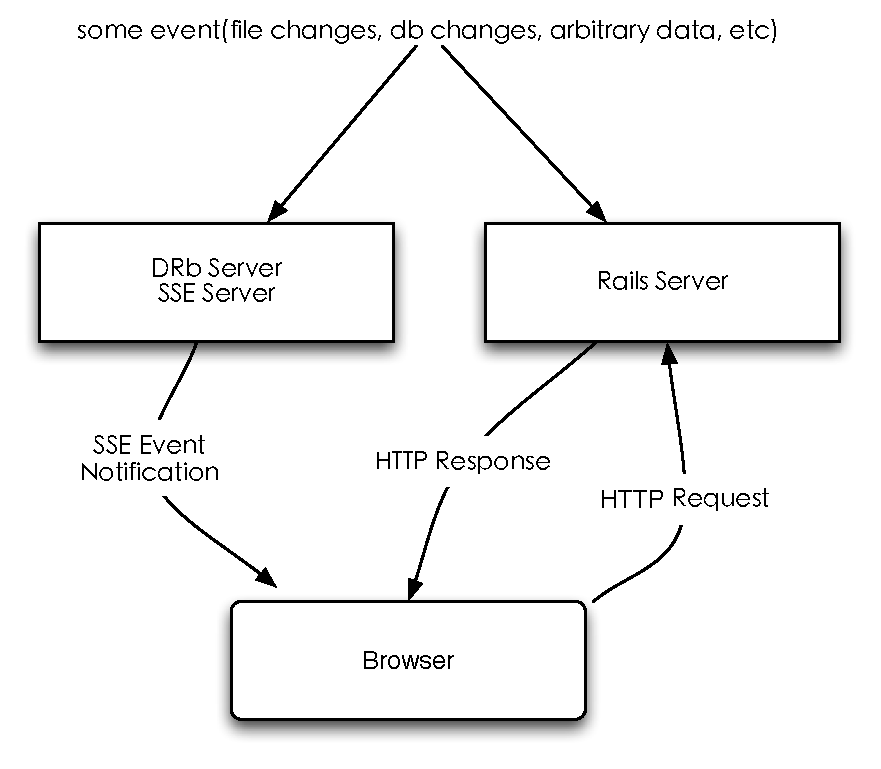
\includegraphics[width=0.7\textwidth]{images/overview/infrastructure.eps}
\caption{基础设施宏观示意图}
\label{fig-infra}
\end{figure}

在图\ref{fig-infra}中,可以看到,Rails消息总线技术主要涉及两方,共4大部件。在图\ref{fig-infra}的最上方是消息源,该部件负责产生消息,并借由Rails消息总线技术将 消息传递给浏览器客户端处。实际上,由于Rails消息总线技术是一门基础性技术,这里的消息源可能是由无数多种组件构成。按照目前实现计划,本文提供了两种消息源:其一是负责监控Rails工程目录下文件的变动,并将关键文件变动消息通知给浏览器客户端,这实际上是Auto-Reload技术的基础;其二则是负责对Rails服务器性能参数进行监控和收集统计,并将这些性能数据实时的传送至浏览器客户端,这实际上是Backend Instrumentation的技术基础。当然,数据源的种类不仅如此。实际上开发者还可以实现数据库的变动监控,一旦发觉数据库内的数据发生变动(比如通过Rails控制台改变),将立刻通知浏览器客户端进行刷新操作,从而即刻反映出后台数据库的变化对前端的影响。

第二大部件则是一个DRb Server组件。在一个典型的网页服务器后端,为了保证服务器的可用性及性能,开发者往往会使用服务器集群,用来均摊高昂的服务器压力,增强服务器的性能表现。同时,服务器后台一般是一个高并发的环境,可能有许多非服务器的进程作为工作子进程而工作。而这些工作子进程在处理用户请求之后,很有可能需要发送实时消息至用户的浏览器。考虑到操作系统进程间天然的隔离性,由于和用户的浏览器客户端通信的实体实际上是服务器进程,因此一般来说非服务器进程往往很难直接和浏览器之间进行通信。这个限制是和Rails消息总线的设计初衷箱违背的。为了解决这个问题,Rails消息总线技术引入了DRb Server部件。该部件负责后台中服务器进程和非服务器进程之间的通信,从而使得非服务器进程能够委托服务器进程向浏览器客户端发送相应的实时消息。

DRb Server不会直接和浏览器客户端通信,它会使用SSE Server模块向浏览器客户端发送消息。SSE Server的设计目标便是提供一套标准的、健壮的服务器到浏览器通信机制。它提供了两套模式,其一是Raw Streaming模式,用于直接向客户端发送原始数据,另一个是SSE Mode,用于和客户端使用HTML5 SSE标准协议进行通信,其稳定性和健壮性要优于前者。

最后,为了使得整个机制能够运转正常,还需要浏览器客户端方面的支持。实际上,第四大部件严格意义上来讲并不属于Rails消息总线技术。它实际上是位于浏览器客户端中的JavaScript脚本,用于接收SSE消息,并且指导浏览器针对不同的消息产生不同的响应行为。

\subsection{SSE Server总体方案设计}
SSE负责和浏览器直接通信,并且能够支持实时的向浏览器传送数据。但是,由于Rails使用了Rack技术(一种服务器通用接口技术),使得Rails很难绕过Rack的限制,直接和浏览器客户端进行通信。不难发觉,为了实现数据能够实时的发送至浏览器客户端,传统的基于Rack技术的网页服务器响应流程已经不适用了,需要一种新的机制来实现之。幸运的是,Rack在1.5之后提出了一套新的服务器接口标准,使得开发者能够直接从Rack手中接手对客户端原始套接字的占有,从而直接操作原始套接字,实现消息的实时发送。为了了解这个技术,需要简要介绍一下经典的Rack服务器响应流程。典型的Rails服务器栈如图\ref{fig-server-stack}所示。

\begin{figure}[h]
\centering
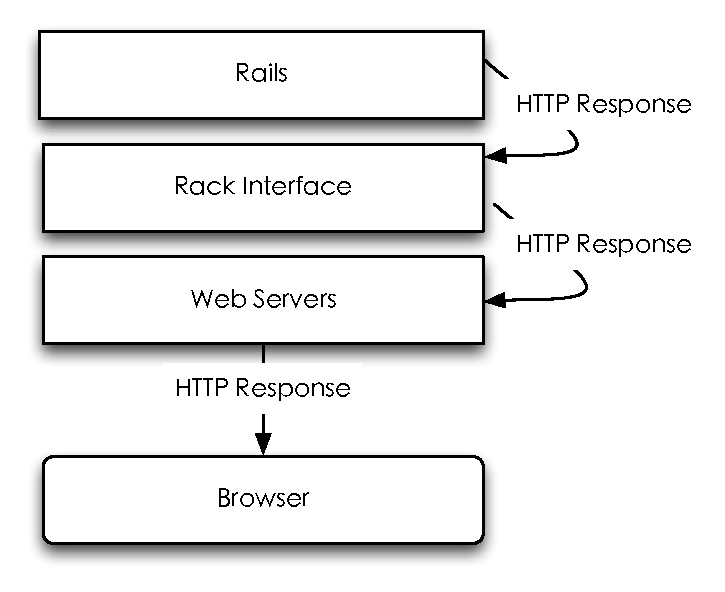
\includegraphics[width=0.7\textwidth]{images/overview/rack.eps}
\caption{典型的Rails服务器栈结构}
\label{fig-server-stack}
\end{figure}

在图\ref{fig-server-stack}中,可以看到,整个Rack技术是基于一种类似于堆栈的组织方式的。在这个服务器堆栈上,位于最顶端的是Rails服务器,其下则是Rack库代码,在之下则是各式各样的Web服务器。Rack技术的提出,主要便是为了解决开发者对代码精简的诉求和种类繁多的Web服务器接口之间的矛盾。Rack抽象出了一套基本的Web服务器接口,使其上层逻辑直接这套接口打交道。在下层,则是针对大量的不同服务器开发了为数众多的服务器适配接口。这样,使用Rack,开发者仅需要针对Rack的接口开发程序,便使得自己的程序能够兼容众多其他的服务器。

图\ref{fig-server-stack}展示了一套典型的Rack


\subsection{DRb Server总体方案设计}

\subsection{Auto Reload总体方案设计}

\subsection{Backend Instrumentation总体方案设计}

\section{系统逻辑结构设计}
根据3.2的解决⽅方案归纳出各种实体类(系统静态结构)描述类之间的交互(系统动态结构)

\section{系统物理结构设计}
本系统开发部署环境(主要是软件环境)本系统得部署图(哪⼀一部分运⾏行在哪⾥里?)